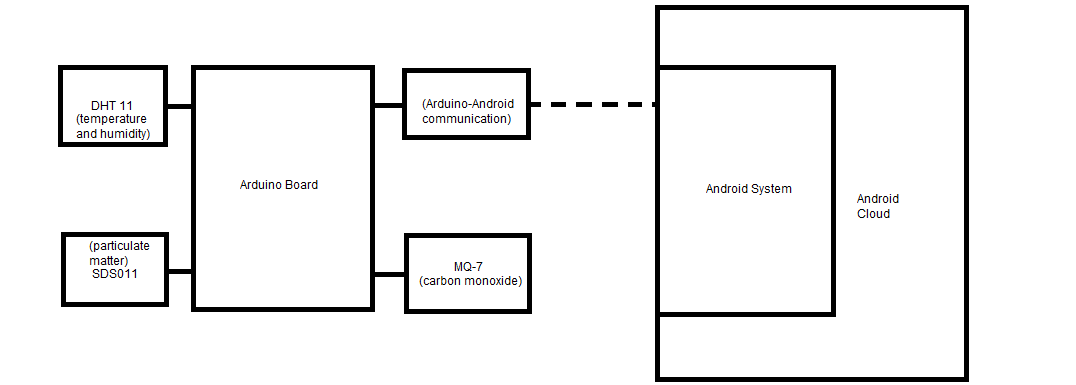
\includegraphics{BlockDiagram}

\begin{center}
Figure 4.1. System Model of the Project
\end{center}

\begin{center}
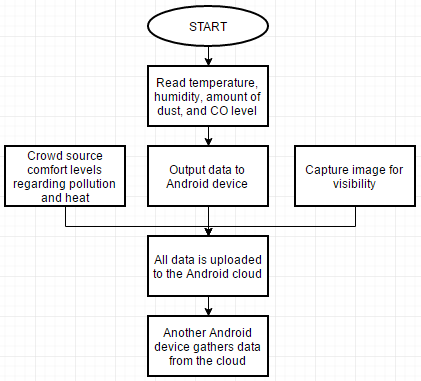
\includegraphics[width=\textwidth]{Flowchart}
\end{center}




\begin{center}
Figure 4.2. System Flowchart
\end{center}

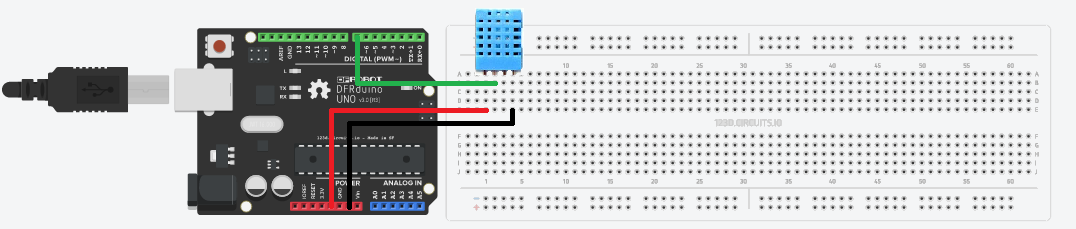
\includegraphics{CurrentProgress}

\begin{center}
Figure 4.3. Circuit Configuration for Testing the DHT-11
\end{center}







\begin{lstlisting}
#include "DHT.h"
#include <LiquidCrystal.h>
LiquidCrystal lcd(12, 11, 5, 4, 3, 2);

const int analogInPin0 = A0;// Analog input pins

#define DHT11_PIN 7

float sensorValue0,sensorValue1 = 0;
float voltageValue0, voltageValue1 = 0;

char inbyte = 0;

DHT dht(7,DHT11);
void setup(){
  lcd.begin(16, 2);
    Serial.begin(9600);
}
void loop()
{
//  int chk = DHT.read11(DHT11_PIN);
  lcd.setCursor(0,0); 
  lcd.print("Temp: ");
  float t = dht.readTemperature();
//  Serial.print("Temp: ");
//  Serial.println(t);
  
  lcd.print(t);
  lcd.print((char)223);
  lcd.print("C");
  lcd.setCursor(0,1);
  float h = dht.readHumidity();

//  Serial.print("Hum: ");
//  Serial.println(h);
  
  lcd.print("Humidity: ");
  lcd.print(h);
  lcd.print("%");
  delay(5000);
  float di = t - 0.55* (1-0.01*h)*(t-14.5);

//  Serial.print("DI: ");
//  Serial.println(di);

  lcd.clear();
  lcd.setCursor(0,0);
  lcd.print("Discomfort Index");
  lcd.setCursor(0,1);
  lcd.print(di);

  delay(2000);
  
  sendAndroidValues(t,h,di);
      lcd.clear();
}

void sendAndroidValues(float t, float h, float di)
 {
  //puts # before the values so our app knows what to do with the data
  Serial.print('#');
  //for loop cycles through 4 sensors and sends values via serial
  
    Serial.print(t);
    Serial.print('+');
    Serial.print(h);
    Serial.print('+');
    Serial.print(di);
    Serial.print('~');
    //technically not needed but I prefer to break up data values
    //so they are easier to see when debugging
 Serial.println();
 delay(10);        //added a delay to eliminate missed transmissions

\end{lstlisting}


\begin{center}
Figure 4.4. Code for Temperature and Humidity Gathering with Bluetooth Transmission
\end{center}


This code is to be utilized in using the DHT-11 sensor in getting the humidity and temperature. This code is file that is part of the DHT library for Arduino systems.

\begin{center}
\begin{eqnarray}
DI = T-0.55(1-0.01H)(T-14.5)
\label{Discomfort Index}
\end{eqnarray}
\end{center}
\begin{center}
Figure 4.5. Formula for Discomfort Index
\end{center}

This is the formula from \cite{Calculator} that is used to calculate the discomfort index where DI is the discomfort index, T is the temperature, and H is the humidity.

\section{Summary}

According to the system model, the project will make use of an Arduino microcontroller system that will handle tasks of gathering inputs which are the temperature, humidity, amount of dust, and amount of carbon monoxide. These data will be transmitted an Android system. Afterwards, this data can be submitted  to the Android cloud in real time. Each individual Android system in the cloud can make use of the camera to capture the image of the surroundings in order to get the visibility with the aid of computer vision. A crowdsourcing element is considered to be added in each system where the user can rank the amount of discomfort he feels in terms of the heat and air pollution. This information will be utilized in the cloud.

The current accomplishments for the group is the successful gathering of the temperature and humidity with the use of the Arduino system and the DHT-11 sensor, the use of the Bluetooth module for transmission, and the development of the Android application. 